\titre{29}
\theme{trigo}
\auteur{Nathan Scheinmann}
\niveau{1M}
\source{sesamath-1M-trigo}
\type{serie}
\piments{2}
\pts{}
\annee{2425}

\contenu{
\tcblower
\begin{minipage}[t]{0.4\textwidth}{
\vspace{0pt}
On considère le triangle $\widehat{MST}$ tel que $\overline{MS}=23~\text{cm}$ et $\overline{TM}=15~\text{cm}$. Les droites $AH$ et $MS$ sont parallèles.
}
\end{minipage}
\hfill
\begin{minipage}[t]{0.55\textwidth}{
\vspace{0pt}
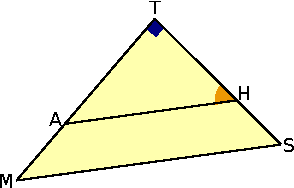
\includegraphics[scale=1]{../medias/1M/trigo/1M-exo-29}
}
\end{minipage}
\begin{tasks}(1)
	\task Écrire les rapports de longueurs qui sont égaux en justifiant.
	\task Écrire la relation donnant le sinus de l'angle $\widehat{AHT}$. 
	\task Déduire des questions précédentes la mesure arrondie au degré près de l'angle $\widehat{AHT}$.
\end{tasks}
}
\correction{

}

